% !TEX root = sum1.tex
\section{Problem Description}
In this section, to incorporate the social distancing into seat planning, we first give the description of the seat planning problem with social distancing. Then we introduce the dynamic seat assignment problem with social distancing.

% dynamic seat assignment problem, which is suitable for commercial use in cinemas and concerts.

\subsection{Seat Planning Problem with Social Distancing}\label{dynamic_demand}
We consider a layout comprising $N$ rows, with each row containing $S_j$ seats, where $j \in \mathcal{N}$. The seating arrangement is intended for various groups, where each group consists of no more than $M$ individuals. There are $M$ distinct group types, denoted by group type $i$ containing $i$ people, where $i \in \mathcal{M} \coloneqq {1,2, \ldots, M}$. Represented by a demand vector $\mathbf{d} = [d_1, \ldots, d_M]$, each element $d_i$ represents the number of group type $i$.


In order to comply with the social distancing requirements, individuals from the same group may sit together, while maintaining a distance from other groups. Let $\delta$ denote the social distancing measure, which could entail leaving one or more empty seats. Specifically, each group must ensure that there are empty seat(s) between them and adjacent groups. Importantly, the seating arrangement of different rows does not affect each other, meaning that individuals from one group can be seated directly behind individuals from another group.

To incorporate the social distancing requirements into the seat planning process, we adjust the original group sizes by adding $\delta$. Consequently, the new size of group type $i$ is denoted as $n_i = i + \delta$, where $i \in \mathcal{M}$. Similarly, to accommodate the adjusted group sizes, the seat layout is modified by adding $\delta$ to the length of each row. Thus, $L_j = S_j + \delta$ represents the length of row $j$, where $S_j$ indicates the number of seats in row $j$. By incorporating the additional seat(s) and designating certain seat(s) for social distancing, we can integrate social distancing measures into the seat planning problem.

% We consider the social distancing of one empty seat throughout the rest of this paper, which is more practical and reasonable in the seat planning. However, our methods are still applicable to the social distancing of two or more seats.


Next, we will analyze the impact of implementing social distancing on each row. We define seat planning as the arrangement of seats within a row, specifically, the number of different groups present in each row. To simplify the discussion, we will use a vector $P_k = (t_1, \ldots, t_M)$ to represent pattern $k$, where each element corresponds to the seat planning for a specific group type.

To quantify the effect of each pattern, we introduce the notion of "loss." Here, the term "loss" denotes the number of individuals that cannot be accommodated due to the implementation of social distancing measures, compared to a scenario without social distancing.

For a given pattern $k$, we denote the loss as $l(k)$. The loss provides a measure of the number of people who cannot be seated due to social distancing constraints. By examining the losses associated with different patterns, we can assess the effectiveness of various seat planning configurations with respect to accommodating the desired number of individuals while adhering to social distancing requirements. 

In cases where the length of a row is fixed, we refer to the patterns with the minimal loss as the "largest" patterns. These largest patterns are characterized by having the least number of people unable to be seated due to social distancing requirements. Furthermore, we classify patterns that have no empty seats, except for those required for social distancing, as "full" patterns. These full patterns are designed to maximize seating capacity while still maintaining the necessary spacing between groups.

By distinguishing the largest and full patterns from other configurations, we can gain valuable insights into the most efficient seat planning strategies that prioritize accommodating the maximum number of people while adhering to social distancing guidelines.

In scenarios where the demand for seating is high, it is advantageous to adopt the largest pattern, as it allows for the accommodation of a larger number of individuals. The largest pattern becomes particularly beneficial when the demand exceeds the capacity of full patterns.

Conversely, when the demand is moderate or not excessively high, adopting the full pattern becomes more feasible. The full pattern maximizes seating capacity by utilizing all available seats, except those required for social distancing measures. By adopting the full pattern, we strive to accommodate as many people as possible while still maintaining the necessary spacing between groups.

Overall, by considering both the largest and full patterns, we can optimize seat planning configurations to efficiently accommodate a significant number of individuals while adhering to social distancing guidelines.

\begin{lem}\label{lem_pattern}
  When given the length of a row, $L$, the social distancing, $\delta$, the adjusted size of the largest group allowed, $n_M$, the loss of the largest pattern is $\lfloor \frac{L}{n_M} \rfloor \delta - \delta + \mathbb{1}(L - \lfloor \frac{L}{n_M} \rfloor n_M)$, where $\mathbb{1}(r)=0$ if $r> \delta$, and $\mathbb{1}(r)= r$ if $r \leq \delta$.
\end{lem}

\begin{example}
  Suppose that the social distancing requirement is one seat, and there are four types of groups. In this case, the new sizes of the groups would be 2, 3, 4, and 5, respectively. Additionally, the length of a single row is determined to be L = 21. 
  
  We find that the patterns (0, 0, 0, 4), (0, 0, 4, 1), and (0, 2, 0, 3) are the largest patterns with the same loss value of 5. However, it's important to note that the largest pattern may not necessarily be a full pattern. For instance, the pattern (0, 0, 0, 4) is the largest pattern in terms of accommodating the maximum number of individuals, but it does not meet the requirement of fully utilizing all available seats since $4 \times 5 \neq 21$.
  
  Conversely, a full pattern may not always be the largest pattern. For example, the pattern (1, 1, 4, 0) is considered a full pattern since it utilizes all seats, but its loss value is 6.
\end{example}


% Therefore, it is crucial to consider both the largest and full patterns separately, as they represent different trade-offs. While the largest pattern maximizes the number of accommodated individuals, the full pattern aims to utilize all available seats. By carefully evaluating these patterns, we can make informed decisions that optimize seat planning configurations while minimizing the loss of seating capacity.

% Then we can illustrate the seat planning for one row below. 
% \begin{figure}[ht]
%     \centering
%     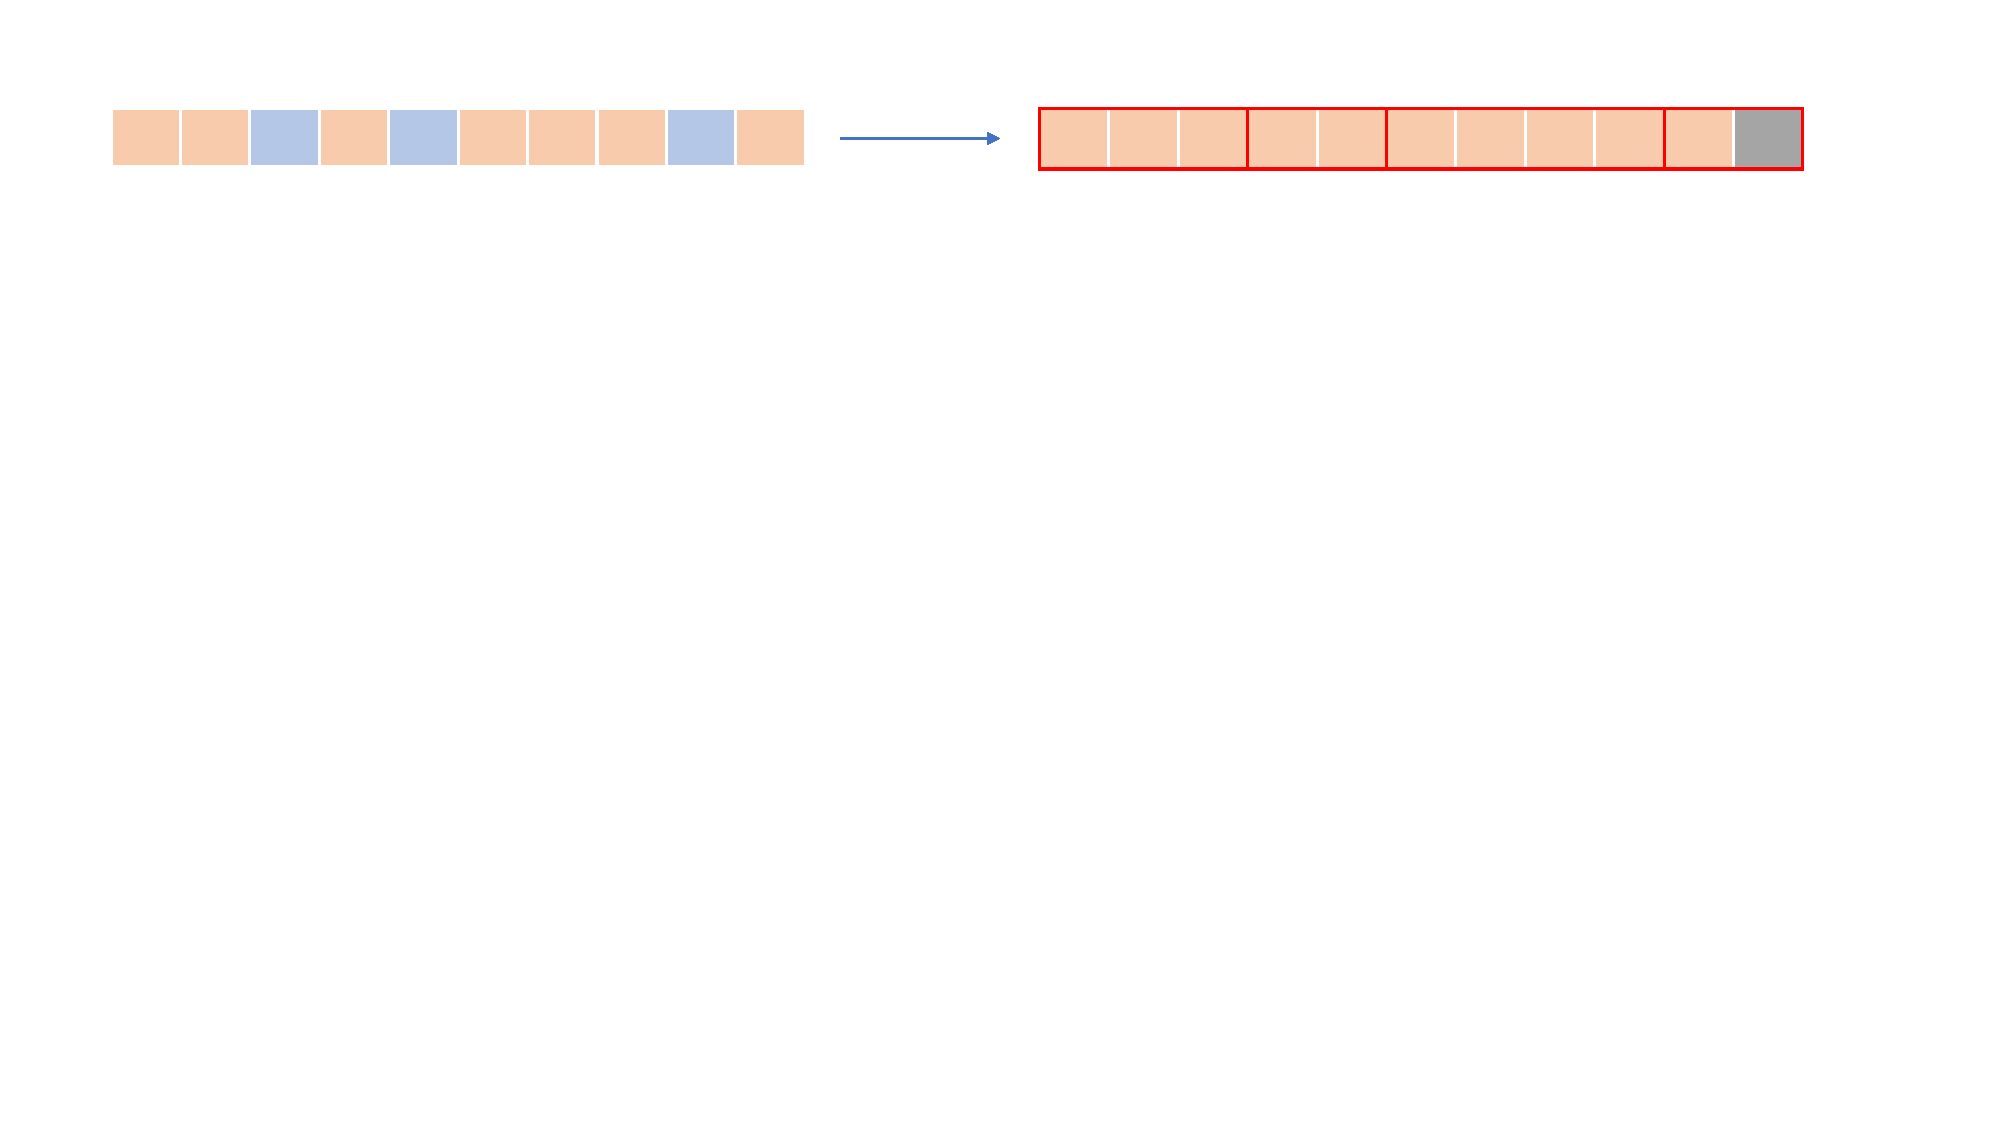
\includegraphics[width = 0.8\textwidth]{./Figures/dummy_seat.pdf}
%     \caption{Problem Conversion}
% \end{figure}

% The social distancing here is one seat. On the left side of the diagram, the blue squares represent the empty seats required for social distancing, while the orange squares represent the seats occupied by groups. On the right side, we have added one dummy seat at the end of each row. The orange squares surrounded by the red line represent the seats taken by groups in this row, which includes two groups of 1, one group of 2, and one group of 3.

% To represent a pattern with a fixed length of form, we can use a $(M+1)-$dimensional vector with $M$ group types. The aggregated form can be expressed as $[n_0, n_1, \ldots, n_M]$, where $n_i$ is the number of $i$-th group type, $i \in \mathcal{M}$. $n_0$ is the number of left seat, its value can only be $0, 1$ because two or more left seats will be assigned to groups. Thus the pattern, $[1, 0, 0, 0, 4]$, is not full because there is one left seat.


% \begin{prop}
% For the seat layout, $\{L_1, L_2, \ldots, L_{N}\}$, the minimal total loss is $\sum_{j} (\lfloor \frac{L_j}{n_{M}} \rfloor \delta -\delta + f(L_j \mod n_{M}))$. The maximal number of people assigned is $\sum_{j} (L_j - \lfloor \frac{L_j}{n_{M}} \rfloor - f(L_j \mod n_{M}))$.
% \end{prop}

\subsection{Dynamic Seat Assignment with Social Distancing}\label{sec_dynamic}
We address the problem of dynamic seat assignment with social distancing, which involves the real-time allocation of seats to incoming groups while ensuring adherence to social distancing guidelines. The decision-maker must make accept or reject decisions for each group and assign them to available seats in rows, while guaranteeing the required spacing between groups. Recalling the seat layout, it consists of $N$ rows, with each row having a length denoted by $L_j$. Additionally, there are $M$ distinct group types.

To model this problem, we adopt a discrete-time framework. The time is divided into $T$ periods, with exactly one group request occurring in each period. Time is discretized as $1, \ldots, T$, where 1 represents the beginning of the selling horizon, and T represents the end. In each period $t$, a group of size $i$ arrives with a probability denoted as $p_i$. The arrivals of different group types are assumed to be independent. During each period, a decision is made regarding whether to accept or reject the incoming group and which row to assign them to. Once seats are confirmed and assigned to a group, they cannot be changed.

To keep track of the remaining capacity of rows, we use a vector $\mathbf{L} = (l_1, l_2, \ldots, l_N)$, where $l_j$ represents the number of remaining seats in row $j$. Let $V_t(\mathbf{L})$ denote the maximal expected value to go at period $t$ with capacity $\mathbf{L}$. Let $u_{i,j}$ denote the decision, where $u_{i,j}(t) = 1$ if we accept a group type $i$ in row $j$ at period $t$, and $u_{i,j}(t) = 0$ otherwise.

The dynamic programming formula for this problem can be expressed as:

$$V_{t}(\mathbf{L}) = \max_{u \in U(\mathbf{L})}\{ \sum_{i=1}^{M} p_i ( \sum_{j=1}^{N} i u_{i,j} + V_{t+1}(\mathbf{L}- \sum_{j=1}^{N} n_i u_{i,j}\mathbf{e}_j^{\top} ))\}, \mathbf{L} \geq 0, V_{T+1}(\mathbf{L}) =0, \forall \mathbf{L}$$

Here, $\mathbf{e}_j$ represents an N-dimensional unit row vector with $j$-th element being 1. In the above formula, the decision set $U(\mathbf{L})$ represents the feasible set of decisions for a given seat availability $\mathbf{L}$. It is defined as: $U(\mathbf{L}) = \{u_{i,j} \in\{0,1\}, \forall i,j| \sum_{j=1}^{N} u_{i,j} \leq 1, \forall i; n_{i}u_{i,j}\mathbf{e}_j^{\top} \leq \mathbf{L}, \forall i,j \}$ 

Essentially, $U(\mathbf{L})$ represents the feasible assignment decisions, where each group type $i$ can be assigned to at most one row, and the corresponding capacity requirements are satisfied.

Initially, we have $\mathbf{L} = (L_1, L_2, \ldots, L_{N})$. The objective function is $V_1(\mathbf{L})$. By applying the dynamic programming formula, we can recursively compute the optimal value function $V_t(\mathbf{L})$, representing the maximum expected value at time $t$ for a given seat availability $\mathbf{L}$. This approach allows us to make optimal decisions regarding group acceptance and seat assignment in order to maximize the overall value while considering social distancing constraints and group arrival probabilities. However, this leads to the curse of dimensionality due to the numerous seat planning combinations. To avoid this complexity, we propose an approach that directly targets the final seat planning and then formulate a policy to assign arriving groups. To obtain the final seat planning firstly, we develop the scenario-based stochastic programming.


% Specifically, we define the concept of target seating plans deemed satisfactory. In making the dynamic seating plan, we will try to maintain the possibility of achieving one of the target seating plans as much as possible.
